\section{Результати роботи та аналіз}

Тестування проводилось під Linux-based операційними системами на двох ПК. Перший ПК мав процесор Intel i5-2400 з заявленною тактовою частотою 3,1 ГГц. Другий ПК мав процесор AMD A10-6790K з заявленною тактовою частотою 4 ГГц. 

Спершу розглянемо результати роботи бенчмарку при компіляції у 64-бітному режимі на ПК з процесором Intel:

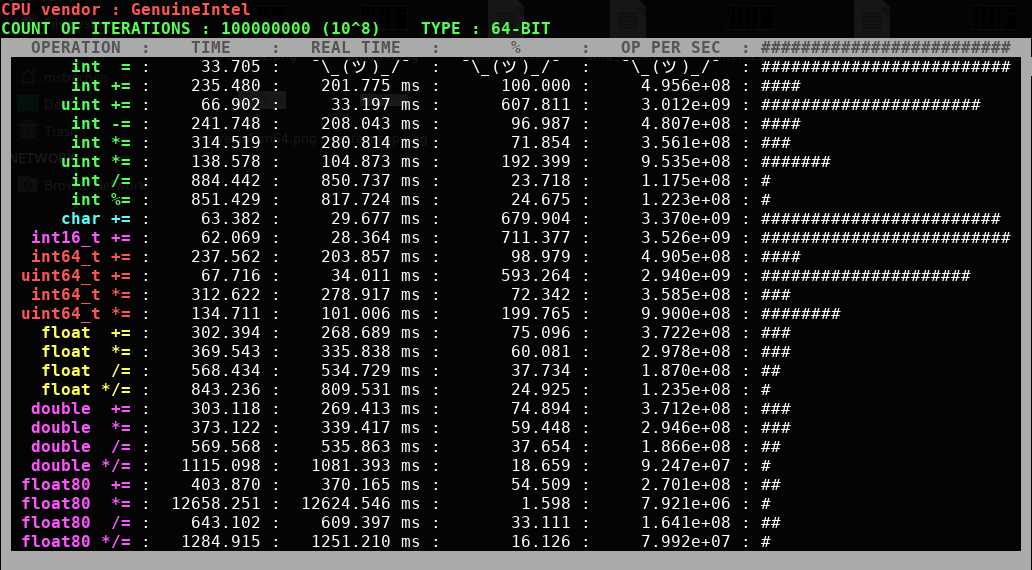
\includegraphics[width = 16cm]{img/intel64.png}

Помітимо деякі цікаві моменти. По-перше, використання беззнакового цілочисельного типу пришвидшує виконання операцій у цілих 6 разів! По-друге, використання 8-ми або 16-бітних цілочисельних типів також дає приріст швидкості у 7 разів. По-третє, різниці у виконанні операцій над 64-бітними і 32-бітними цілими числами немає. 

Порівняємо з результатами роботи бенчмарку у 32-бітному режимі:

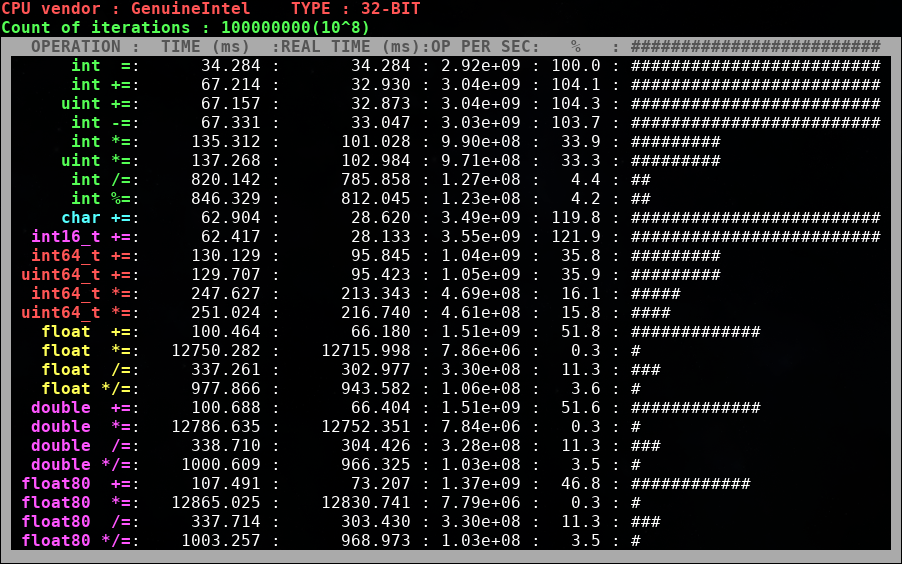
\includegraphics[width = 16cm]{img/intel32.png}

Бачимо, що операції над 64-бітними цілими стали коштувати приблизно вдвічі дорожче відносно 64-бітних цілих. Дуже неприємним моментом є погіршення опрацювання операції множення над дійсними числами. На це є дві причини. Першу причину можна помітити, проаналізувавши результати "просто множення" і "множення + ділення" над дійсними типами данних.  В данному бенчмарку є особливість - при множенні, починаючи з деякої ітерації ми отримуємо у змінній значення inf (через недосконалість збереження данних у цих типах даних). Через це страждає виконанн операції множення (тому що обробка "нескінченності" як окремого випадку займає додаткові ресурси процесора). 
Друга причина криється в особливостях компіляції. Проаналізуємо згенерований асемблерний код.

Ліворуч - вихідний текст на C++, по центру - згенерований код у випадку компіляції з прапорцем -m32, праворуч - у випадку компіляції з прапорцем -m64. 


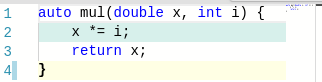
\includegraphics[width = 6cm]{img/screencpp.png}
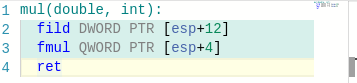
\includegraphics[width = 6cm]{img/screenAsm32.png}
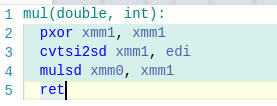
\includegraphics[width = 5cm]{img/screenAsm64.png}

Як бачимо, у випадку компіляції у 32-бітному режимі операції виконуються з оперативною пам'ятю, а ось у випадку 64-бітного режиму усе виконується виключно в регістрах. Регістри при цьому значно швидші за доступом, а тому вітка обробки нескінченних значень у типах з плаваючою комою виконується довше.

Тепер проаналізуємо швидкодію ПК з процесором AMD.

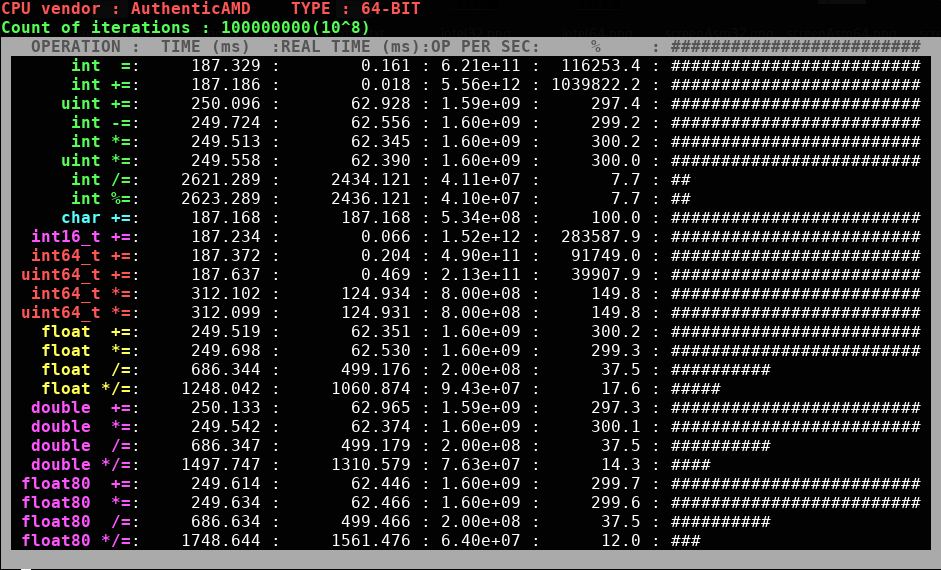
\includegraphics[width = 16cm]{img/amd64.png}

Якщо порівнювати з Intel, то процесор AMD (судячи з бенчмарку) страждає від повільного копіювання (майже вдвічі гірше, ніж у Intel), а також у цілому гірше працює з дійсними типами даних. Якщо бути точнішим, додавання і множення виконується значно гірше для 32- та 64-бітних типів даних. Утім, ділення 32- та 64-бітних дійсних виконується швидше. Ще однією особливістю є швидка робота з 8-бітними цілими (швидше ніж просте копіювання 32-бітних цілих). 

Проаналізуємо також виконання бенчмарку з прапорцем -m32.

Помітна значна деградація швидкодії при роботі з 64-бітними знаковими цілими і помірна деградація при роботі з дійсними типами даних. Крім того, помітний значний приріст швидкодії з 16-бітними цілими (з одночасною деградацією швидкодії з 8-бітними цілими).

(Скріншот результатів бенчмарку наведено на наступній сторінці).

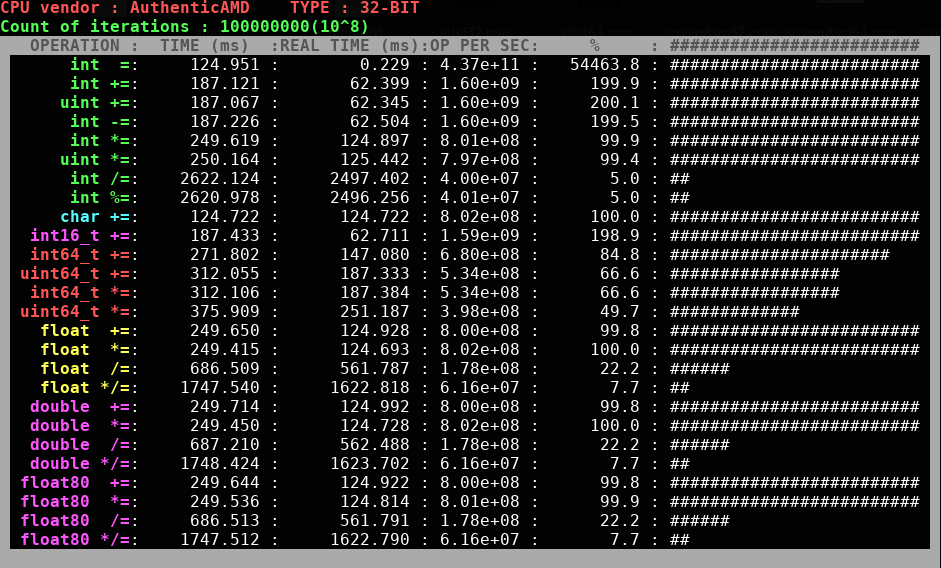
\includegraphics[width = 16cm]{img/amd32.png}
 



